\chapter{Particle Interaction Theory}
\label{chap:particle-interaction-theory}

As mentioned in the introduction.

\paragraph{Definition: An $N_p$-Body System}
is a set of particles with position and velocity interacting with one another.
% \paragraph{Inertia / kinetic energy}
Each particle individually is subject to inertia and its kinetic energy (``second moment'' \footnote{
  In kinetic theory, the $0$th moment is the mass $m_i$ of a particle, the first moment is the momentum $\vec{p_i}$ and the second moment is its kinetic energy $E_{kin,i}$.
}) is given by
$$E_{\text{kin},i} = \frac{\vec{p_i}^2}{2m} = \frac{(m \vec{v_i})^2}{2m} = \frac{1}{2} m \norm{\vec{v_i}}^2\,.$$
The second important ingredient is an interaction potential motivating pairwise forces $\vec{F_{ij}} \in \R^d$ between particles
$$\vec{F}_{ij} = -\nabla U_{ij} = -\left(\partial x_1, ..., \partial x_d\right)^T U_{ij}\,.$$

The total potential of a system of $N_p \ge 2$ particles $U \in \R$ can be calculated by summing up the pair potentials $U_{ij} \in \R$ between all pairs of particles
$$U = \sum_{i=1}^{N_p}\sum_{j=1, j \neq i}^{N_p} U_{ij} = \sum_{i=1}^{N_p}\sum_{j=1, j \neq i}^{N_p} K\left(\norm{\vec{x_i} - \vec{x_j}}\right)\,,$$
where $\vec{x_i} \in \R^d$ represents the $d$-dimensional position of particle $i$, respectively.
An example we will study is that of an attractive-repulsive interaction potential, where two power-law potentials compete with each other.
For a given $\alpha, \beta \in \R \backslash \{0\}$, it is given by
$$K_{\alpha, \beta}(r) = \frac{r^\alpha}{\alpha} - \frac{r^\beta}{\beta}\,.$$
One can even consider the case where either $\alpha$ or $\beta$ is 0 in order to arrive at a log-term \parencite{2017-explicit-solutions}, using the convention that $\frac{x^0}{0} := \log(x)$\footnote{
  Consider the Laurent series expansion of $\frac{x^a}{a} = \frac{1}{a} + \log(x) + \frac{1}{2}a \log^2(x) + \mathcal{O}(a^2)$ in the limit as $a \rightarrow 0^+$.
  While this limit approaches $\infty$ coming from the right and $-\infty$ coming from the left due to the nature of the first term in the expansion, the only remaining term in it is $\log(x)$ which is thereby chosen as a convention.
}.
If the repulsive term is stronger (so $\beta > \alpha$), there is no equilibrium distribution as particles simply continue repelling each other out to infinity.

% Some input from the Wolfson Particle Physicist
The Lennard-Jones potential ($\alpha=-12, \beta=-6$), for example, is an \textbf{intermolecular} potential, so the relevant length-scale is between molecules.
Therefore, the only relevant interaction is the electromagnetic force.
Other forces, such as strong force which keeps protons in the nucleus together (a force much stronger than the electromagnetic one, but with much lower reach), need not be considered at this length-scale.

In the absence of an external potential $V$, the total energy is given by $E = E_{\text{kin}} + U$, so
\begin{equation}
  E = \frac{1}{2} \sum_{i=1}^{N_p} m_i \vec{v_i}^2 + \sum_{i=1}^{N_p}\sum_{j=1, j \neq i}^{N_p} K\left(\norm{\vec{x_i} - \vec{x_j}}\right)\,.
  \label{eq:total-energy}
\end{equation}

Each particle $i=1, ..., N_p$ at position $\vec{x_i} \in \R^d$ and time $t \in \R^+$ then follows
\begin{equation}
  \frac{\dd^2 \vec{x_i}}{\ddt^2} = f\left(\norm{\frac{\dd \vec{x_i}}{\ddt}}\right) \frac{\dd\vec{x_i}}{\ddt} - \frac{1}{N} \sum_{j=1, i\neq j}^{N} \nabla K\left(\norm{\vec{x_i} - \vec{x_j}}\right)\,,
  \label{eq:evolution-equation}
\end{equation}
for reference see, for example, \parencite{2020-power-law-kernels, 2021-arbitrary-dimensions}.
For now, we only consider the case without an external potential $V(\vec{x})$.

\section{Continuous Limit}
The evolution equation, in the continuous limit as $N_p \rightarrow \infty$, becomes
\begin{equation}
  \frac{\partial \rho}{\partial t} = \nabla \cdot \left(\rho \nabla K * \rho\right)\,.
  \label{eq:continuous-evolution-equation}
\end{equation}
where $\rho: \R \mapsto \R$ is the particle density function.
\begin{proof}
  \hierKoennteIhreWerbungStehen
\end{proof}
The solution $\rho$ we are looking for within the scope of this dissertation is the \textit{equilibrium measure} (cf. \Cref{def:equilibrium-measure}) minimizing the total potential $U$.

\begin{definition}{Equilibrium Measure}{equilibrium-measure}
  For a given pairwise interaction potential $K: \R \mapsto \R$, the equilibrium measure $\rho: \mathbb{R} \mapsto \mathbb{R}$ is a measure chosen such that
  $$U = \frac{1}{2} \iint K\left(\norm{\vec{x} - \vec{y}}\right) \,\dd\rho(\vec{x})\,\dd\rho(\vec{y})\,,$$
  is minimised, where $\dd\rho = \rho(\vec{x})\dd\vec{x}$.
\end{definition}
Also consider the total mass of the equilibrium distribution, given by
\begin{equation}
  M = \int \dd\rho = \int_{\supp(\rho)} \rho(\vec{x}) \,\dd\vec{x}\,,
  \label{eq:measure-mass}
\end{equation}
which, without loss of generality, we can choose as $M = 1$ to make $\rho(\vec{x})$ a \textit{probability distribution}.

\section{Self-Propulsion}
Makes it active matter.
Self-propulsion and friction could be modelled as a quadratic of the form
$$f(v_i) = 1.6 - 0.5 v_i^2\,,$$
where $v_i := \norm{\vec{v_i}} = \norm{\frac{\dd\vec{x_i}}{\ddt}}$.

\begin{figure}[H]
  \centering
  \label{fig:simulation-quiver-illustration}
  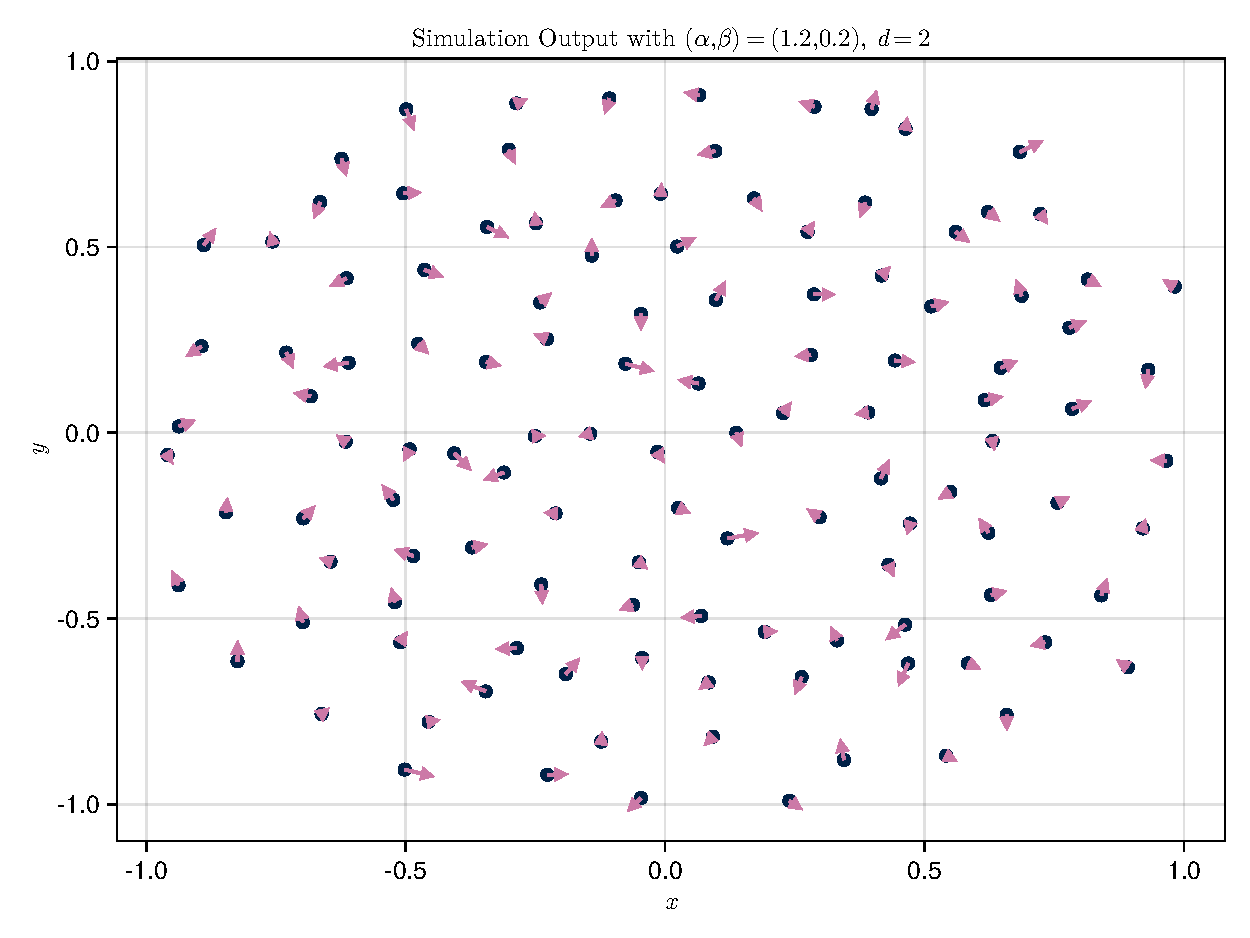
\includegraphics[width=0.8\linewidth]{results/morse-2d/simulation-quiver.pdf}
  \caption[Quiver plot of 120 particles in 2D interacting through the Morse potential]{Position and velocity of $N_p = 120$ particles $d = 2$ dimensions as obtained through the molecular dynamics simulation introduced in \Cref{chap:particle-simulator}. The interaction potential is a Morse potential with given parameters. Friction and self-propulsion terms are present as described in \cite{2006-self-propelled}, so using $f(v_i) = 1.6 - 0.5 v_i^2$, this figure reproduces their results.}
\end{figure}

\hierKoennteIhreWerbungStehen

% TODO: Friction Term -> Energy Dissipation -> Different Plot

\section{Kinetic Theory: The Vlasov Equation}
A very common tool in Plasma physics.
$$\frac{\partial f}{\partial t}+{\frac {\mathrm {d} \mathbf {r} }{\mathrm {d} t}}\cdot {\frac {\partial f}{\partial \mathbf {r} }}+{\frac {\mathrm {d} \mathbf {p} }{\mathrm {d} t}}\cdot {\frac {\partial f}{\partial \mathbf {p} }}=0,$$

This is the collisionless Boltzmann equation.
Vlasov replaces the collision term with long-range interactions.

\begin{theorem}{Liouville's}{liouville}
  Says that phase-space volume is conserved in situations of a pure particle-particle interaction.
  $$\frac{d\rho}{dt}=
    \frac{\partial\rho}{\partial t}
    +\sum_{i=1}^n\left(\frac{\partial\rho}{\partial q_i}\dot{q}_i
    +\frac{\partial\rho}{\partial p_i}\dot{p}_i\right)=0\,.$$
\end{theorem}

\section{Vicsek Model}
For the study of active matter (a number of individual agents).

\section{Swarming}
A 2010 paper by \citeauthor{2010-starlings} showed the surprising result that correlation between movement of individual starlings in bird flocks over Rome is scale-free.
In contrast to the assumption that birds only mirror their neighbours' behaviour and swarming behaviour emerges as a result of that, this observation suggests that bird flocks exert collective behaviour beyond local interactions.
\begin{quote}
  The change in the behavioral state of one animal affects and is affected by that of all other animals in the group, no matter how large the group is
  \parencite{2010-starlings}.
\end{quote}
This work was done by individually tracking each starling in the flock and using tracking algorithms to represent their 3 dimensional positions and velocities.
